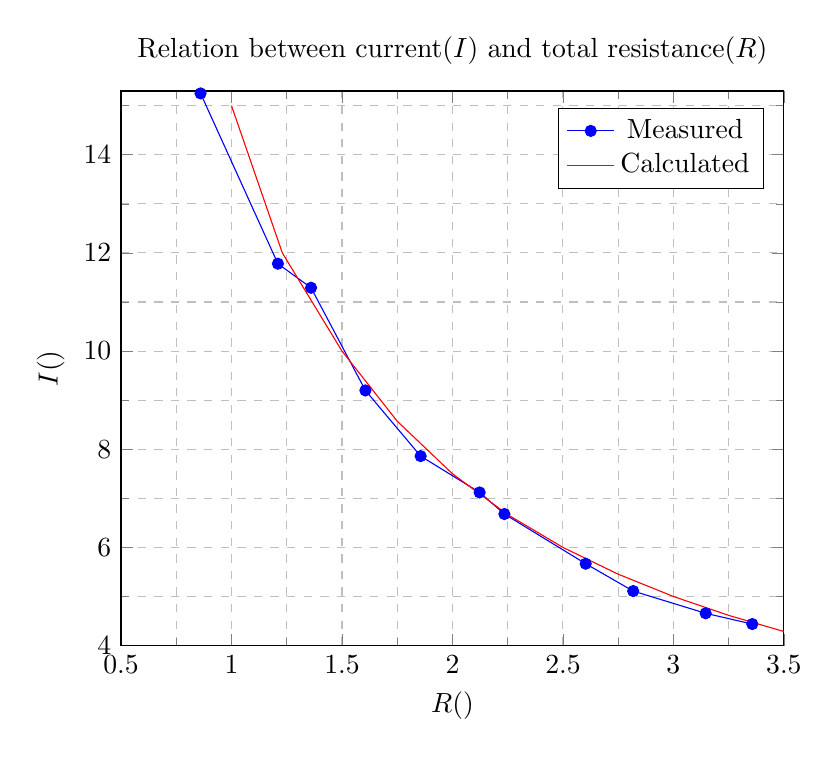
\begin{tikzpicture}
    \begin{axis}[
            title = {Relation between current($I$) and total resistance($R$)},
            width=10cm,
            xlabel= {$R(\si{\kilo\ohm})$},
            ylabel= {$I(\si{\milli\ampere})$},
            xmin=0.5,xmax=3.5,
            ymin=4,ymax=15.3,
            grid = both,
            minor tick num = 1,
            grid style=dashed,
            x tick label style={
                /pgf/number format/.cd,
                set decimal separator={$.$}
            },
            legend pos=north east,
        ]
        \addplot[
            color=blue,
            mark=*,
        ]
            coordinates{
(0.860,15.25)
(1.210,11.78)
(1.360,11.29)
(1.606,9.198)
(1.856,7.86)
(2.123,7.120)
(2.235,6.680)
(2.603,5.667)
(2.818,5.110)
(3.146,4.657)
(3.357,4.438)
                       };
                       \addlegendentry{Measured}
        \addplot[
            color=red,
            mark=,
        ]
            coordinates{
(1,15)
(1.23,12)
(1.5,10)
(1.75,8.571)
(2,7.5)
(2.25,6.667)
(2.5,6)
(2.75,5.454)
(3,5)
(3.25,4.615)
(3.5,4.286)
                       };
                       \addlegendentry{Calculated}
    \end{axis}         
\end{tikzpicture}      
